% !TeX root = ../queens.tex
\section{Computing one queen from local records}\label{sec:local}

We now begin our work on proving $|d_j-j|\le4$ 
(Lemma~\ref{lem:estimates}). 
While the greedy-queens process is deterministic, describing its state 
by the entire configuration of earlier queens gives an infinite 
collection of growing states.
This section introduces a notion of \emph{local state} (Definition~\ref{def:local-state}) 
that tracks only selected information about earlier queens. 
Doing so will allow us to model the entire infinite process using only 
finitely many states. After introducing local states, the rest of this
section details an algorithm (Algorithm~\ref{alg:local-successors}) for how one can use the local state before
column~$n$ to place a queen on column~$n$ and update the state for the
next column. However, since the local state only has partial information
about the board, different configurations of earlier queens may yield the
same local state. Thus the algorithm will sometimes return several possible
next placements and states.

Section~\ref{sec:sufficiency} proves that, if certain conditions hold, then there always 
exists a branch of the algorithm of Section~\ref{sec:local} that agrees with the 
greedy algorithm on where to place the next queen and how to update 
the records.

Section~\ref{sec:finite} then computationally verifies that the initial state of 
the board satisfies those conditions, and that exploring every 
possible successor yields a finite collection of states, all 
satisfying those conditions (the state graph, Definition~\ref{def:state-graph}).
Finally, induction using the results of Section~\ref{sec:sufficiency} proves that
the actual greedy process produces states that always stay
within the state graph.
Together with a direct check of the initial placements,
the conditions imply that $|d_j-j|\le4$ for all lower queen
placements, which proves Lemma~\ref{lem:estimates}.

The next two subsections start our work by introducing the eight
records that comprise a local state. 



\subsection{Testing lower attacks}\label{sec:local-rank}
Imagine that we are now trying to place a queen in column $n$.
We first test if there is a free lower square for our queen to use.
Writing $m\ge1$ for the least unused row and $d\ge1$ for the least 
unused lower-diagonal magnitude, we see that a lower square can
be chosen only if its row lies in $[m\dts n-d]$.
Indeed, all rows below $m$ are used, and the square $(n, n-i)$ lies on 
the $i$th lower diagonal, which is used for $i<d$.
 
Write
\begin{equation}\label{eq:window}
 w=n-m-d,
\end{equation}
so that the lower squares to test are $(n,m+r)$ for offsets $r=0,\dots,w$.
If $w<0$, there are no lower candidates, so the queen in column $n$
is upper. If $w\ge0$, it is possible for all $w+1$ candidate squares
to be attacked, in which case the queen is upper as well.

To test candidates, the local state tracks attacks from lower and upper
queens separately. Upper attack records will be discussed in Section~\ref{sec:upper-word}.
To track lower attacks, the local state maintains three sets $R,D,A$ of
nonnegative integers. Consider all earlier lower queens; that is, lower
queens before column $n$. For each such queen $(x,y)$, its row,
lower-diagonal magnitude, and antidiagonal index are $y$, $x-y$,
and $x+y$. We record their offsets from the reference values $m$,
$d$, and $n+m$, keeping only nonnegative values (as the negative values cannot attack our candidate squares):
\begin{align}
 R&=\{y-m:(x,y)\text{ is an earlier lower queen},\ y\ge m\},\notag\\
 D&=\{x-y-d:(x,y)\text{ is an earlier lower queen},\ x-y\ge d\},
       \label{eq:sets}\\
 A&=\{x+y-(n+m):(x,y)\text{ is an earlier lower queen},\ x+y\ge n+m\}.
       \notag
\end{align}
It follows that
\begin{center}
\begin{tabular}{lll}
\toprule
an earlier lower queen attacks $(n,m+r)$&when&record used\\
\midrule
along its row&$r\in R$&row offset\\
along its diagonal&$w-r\in D$&diagonal offset\\
along its antidiagonal&$r\in A$&antidiagonal offset\\
\bottomrule
\end{tabular}
\end{center}
Since row $m$ and magnitude $d$ are unused, we have
$0\notin R$ and $0\notin D$.

The diagonal discrepancy already has a useful expression in these
records. Suppose the next queen is the $j$th lower queen and it uses
offset $r$, so that it has coordinates $(n,m+r)$. 
Since the $j-1$ previous lower queens have used the $d-1$
magnitudes less than $d$, together with the $|D|$ magnitudes greater than it, it follows that
\begin{equation}\label{eq:local-rank}
 j=d+|D|,\qquad d_j=d+w-r,\qquad
 d_j-j=w-r-|D|.
\end{equation}
In particular, $w\le4$ and $D\subseteq[1\dts4]$ would prove the
desired bound, since whenever a lower queen is chosen, 
both $w-r$ and $|D|$ would then belong to $[0\dts4]$. 
We will establish these bounds in Section~\ref{sec:finite}.



\subsection{Testing upper attacks}\label{sec:upper-word}

We now test if a candidate lower queen $(n,m+r)$ is attacked
by any upper queens. Upper queens cannot attack lower queens
along diagonals, so we only need to test if a lower candidate
is attacked by an upper queen along a row or an antidiagonal.

We first introduce an infinite word that tracks upper rows and columns.

\begin{definition}[Queen word]\label{def:queen-word}
For $i\ge1$, let $u_i=[\text{column $i$ has an upper queen}]=[q_i>i]$ and
$b_i=[\text{row $i$ has an upper queen}]$.
The \emph{queen word} is $\sigma=\sigma_1\sigma_2\dots$, where
its \emph{$i$th symbol}
\[
 \sigma_i=2u_i+b_i\in\{0,1,2,3\}
\]
records whether column $i$ and row $i$ contain upper queens.
We call $u_i$ and $b_i$ the \emph{column bit} and the
\emph{row bit} of $\sigma_i$.
\end{definition}

Before column $n$, the prefix $\sigma_1\dots\sigma_{n-1}$
is determined by the queens already placed: for $i<n$,
column $i$ has been filled, and any upper queen in row $i$
must lie in a column less than $i$.

The local state will store subwords of the queen word from
two locations: near index $m$, for testing the lower candidates;
and near index $n$, for checking the new symbol $\sigma_n$
produced at the current step.
The records maintained at these two indices are
\[
 \begin{array}{ll}
 \text{the input history}&H_{\mathrm{in}}=\sigma_{m-12}\dots\sigma_{m-1},\\
 \text{the queue}&Q=\sigma_m\dots\sigma_{m+|Q|-1},\\
 \text{the output history}&H_{\mathrm{out}}=\sigma_{n-12}\dots\sigma_{n-1}.
 \end{array}
\]
The queue $Q$ is a nonempty subword beginning at index $m$.
Unlike the two twelve-symbol histories, its length may vary.

We introduce one final record. The upper-queen tests of
Section~\ref{app:upper} compare positions of upper queens with
positions involving the current column. By Lemma~\ref{lem:upper},
the upper queen in column $c$ has row $c+U(c)$, which involves the
growing count $U$. The state records the single quantity
\[
 z=n-m-U(m-1),
\]
which Section~\ref{app:upper} shows is enough to make these
comparisons. Together with the records from
Section~\ref{sec:local-rank}, we get the eight fields that comprise
a local state:

\begin{definition}[Local state]\label{def:local-state}
A (local) \emph{state} is a tuple
\begin{equation}\label{eq:state}
 (w,z,R,D,A,H_{\mathrm{in}},Q,H_{\mathrm{out}}).
\end{equation}
Here $w,z$ are integers, $R,D,A$ are finite sets of nonnegative
integers, $H_{\mathrm{in}},H_{\mathrm{out}}$ are words of length
twelve over $\{0,1,2,3\}$, and $Q$ is a nonempty word over the
same alphabet. On an actual partial board, the fields have the
meanings discussed in Section~\ref{sec:local-rank} and this subsection;
but we also allow states that do not correspond to actual board
configurations.
\end{definition}
Note that the absolute indices $n,m,d$ are not stored in the local state.
As a concrete example of a state, immediately before column $n=41$,
we have $m=25$, $d=14$, and $U(24)=16$, so
\[
 w=n-m-d=2,\qquad z=n-m-U(m-1)=0,\qquad
 R=A=\varnothing,\quad D=\{1,2\}.
\]
Here $H_{\mathrm{in}}=\sigma_{13}\dots\sigma_{24}=\texttt{212223003223}$,
$Q=\sigma_{25}\dots\sigma_{29}=\mathtt{01212}$, and
$H_{\mathrm{out}}=\sigma_{29}\dots\sigma_{40}=\texttt{212203230303}$.
% Thus $Q$ and $H_{\mathrm{out}}$ share the symbol $\sigma_{29}$.
The lower candidates are rows $(m,\dots,m+w)=(25,26,27)$. Their symbols
$\sigma_{25}\sigma_{26}\sigma_{27}=\texttt{012}$ have row bits
$b_{25}b_{26}b_{27}=\texttt{010}$. Thus the candidate $(41,26)$ is attacked along its row
by an upper queen. Figure~\ref{fig:state-portrait} shows all eight records.
\begin{figure}[!b]
\centering
\setlength{\abovecaptionskip}{0pt}
\begin{tikzpicture}[x=1cm,y=1cm,font=\footnotesize,>=stealth]
 \node[anchor=west,font=\small] at (.2,4.8) {The board before column $41$};
 \node[anchor=west,font=\small] at (6.5,4.8) {The lower attack records};
 \begin{scope}[shift={(.75,1.15)},x=.51cm,y=.51cm]
  \setboardfontsize{13pt}
  \foreach \xx in {0,...,5} \foreach \yy in {0,...,6} {
   \pgfmathtruncatemacro{\parity}{mod(\xx+\yy,2)}
   \ifnum\parity=0 \fill[black!4] (\xx-.5,\yy-.5) rectangle (\xx+.5,\yy+.5);\fi
  }
  \fill[queensLower!13] (3.5,2.5) rectangle (4.5,5.5);
  \draw[black!50] (4,-.5)--(4,6.5);
  \draw[queensLower!55,densely dashed] (-.5,.5)--(5.4,6.4);
  \draw[queensLower,thick] (0,0)--(4.45,4.45);
  \draw[queensLower,thick] (2,1)--(4.45,3.45);
  \draw[queensUpper,dashed] (-.5,4)--(4.5,4);
  \node[text=queensLower,inner sep=0pt] at (0,0) {\BlackQueenOnWhite};
  \node[text=queensLower,inner sep=0pt] at (2,1) {\BlackQueenOnWhite};
  \foreach \yy in {3,4,5} \node[queensLower] at (4,\yy) {$\times$};
  \node[anchor=east,text=queensLower] at (1.05,2.5) {$d=14$};
  \node[anchor=west] at (4.6,3) {$m=25$};
  \node[anchor=west] at (4.6,5) {$27$};
  \draw[<->,black!65] (7.85,3)--(7.85,5);
  \node[anchor=west] at (8.05,4) {$w=2$};
  \foreach \xx/\lab in {0/37,2/39,4/41}
   \node[anchor=north,text=black!65] at (\xx,-.7) {$\lab$};
  \node[anchor=south,queensUpper,font=\scriptsize] at (1.2,4.08) {upper row $26$};
 \end{scope}
 \draw[->,black!45] (5.15,2.3)--(6.05,2.3);
 \node[align=center,text=black!60,font=\scriptsize] at (5.6,1.77) {record\\offsets};
 \foreach \yy/\letter/\recset in {4.05/R/\varnothing,2.75/D/{\{1,2\}},1.45/A/\varnothing} {
  \node[anchor=west] at (6.5,\yy) {$\letter=\recset$};
  \draw[->,black!35] (9.25,\yy)--(14.3,\yy);
  \foreach \i in {0,...,4} {
   \draw[black!40] ({9.6+.9*\i},\yy-.08)--({9.6+.9*\i},\yy+.08);
   \node[anchor=south,font=\scriptsize,text=black!65] at ({9.6+.9*\i},\yy+.12) {$\i$};
  }
 }
 \foreach \i in {1,2}
  \filldraw[fill=queensLower!25,draw=queensLower] ({9.6+.9*\i-.16},2.59) rectangle ({9.6+.9*\i+.16},2.91);
 \node[anchor=west,text=black!60,font=\scriptsize] at (6.5,3.62) {rows measured from $m=25$};
 \node[anchor=west,text=black!60,font=\scriptsize] at (6.5,2.32) {magnitudes $15,16$, measured from $d=14$};
 \node[anchor=west,text=black!60,font=\scriptsize] at (6.5,1.02) {antidiagonals measured from $n+m=66$};
 \draw[black!15] (.2,.12)--(14.4,.12);
 \node[anchor=west,font=\small] at (.2,-.3) {The upper-word records};
 \node[anchor=west,font=\scriptsize,text=black!80] at (.2,-.72) {$z=n-m-U(m-1)=41-25-16=0$};
 \node[anchor=east,text=black!60,font=\scriptsize] at (14.4,-.3) {filled cell $=1$; empty cell $=0$};
 \begin{scope}[yshift=-.45cm]
 % Columns 13,...,40; the symbol at 29 belongs to both Q and H_{\mathrm{out}}.
 \foreach \s [count=\j from 0] in {2,1,2,2,2,3,0,0,3,2,2,3,0,1,2,1,2,1,2,2,0,3,2,3,0,3,0,3} {
  \pgfmathtruncatemacro{\ub}{floor(\s/2)}
  \pgfmathtruncatemacro{\bb}{mod(\s,2)}
  \ifnum\ub=1 \def\ucolor{queensUpper!55}\else\def\ucolor{white}\fi
  \ifnum\bb=1 \def\bcolor{queensUpper!55}\else\def\bcolor{white}\fi
  \filldraw[fill=\ucolor,draw=black!25,line width=.25pt] ({2.7+.39*\j},-1.4) rectangle ({3.09+.39*\j},-1.04);
  \filldraw[fill=\bcolor,draw=black!25,line width=.25pt] ({2.7+.39*\j},-1.9) rectangle ({3.09+.39*\j},-1.54);
 }
 \node[anchor=east] at (2.45,-1.22) {upper column $u_i$};
 \node[anchor=east] at (2.45,-1.72) {upper row $b_i$};
 \foreach \j/\lab in {0/13,12/25,16/29,27/40}
  \node[anchor=north,text=black!60,font=\scriptsize] at ({2.895+.39*\j},-2.02) {$\lab$};
 \draw[decorate,decoration={brace,amplitude=4pt},black!65] (8.94,-.86)--(13.62,-.86);
 \node at (11.28,-.52) {$H_{\mathrm{out}}$};
 \draw[decorate,decoration={brace,mirror,amplitude=4pt},black!65] (2.7,-2.48)--(7.38,-2.48);
 \node at (5.04,-2.88) {$H_{\mathrm{in}}$};
 \draw[decorate,decoration={brace,mirror,amplitude=4pt},black] (7.38,-2.48)--(9.33,-2.48);
 \node[text=black] at (8.355,-2.88) {$Q$};
 \draw[black!55] (7.38,-1)--(7.38,-1.94);
 \draw[->,black!55] (13.95,-2.45)--(13.95,-1.9);
 \node[anchor=north,text=black!65,font=\scriptsize] at (13.95,-2.52) {$n=41$};
 \end{scope}
\end{tikzpicture}
\par\nointerlineskip
\caption{The eight records $(w,z,R,D,A,H_{\mathrm{in}},Q,H_{\mathrm{out}})$ of the local state before column $41$.}
\label{fig:state-portrait}
\end{figure}


The separation into lower attack records and information about
upper queens is closely related to Carter's reduced description
\cite[Section~5]{Carter}.


\subsection{The history graph}\label{app:graph}
Given a state before column $n$, we use the term 
\emph{calculation} to refer to
the algorithm outlined at the start of this section: it chooses the
queen in column~$n$, produces the new symbol $\sigma_n$, and updates
the eight records for column $n+1$. It reads only the stored records
and the history graph defined below, so it can be carried out on any
state, whether or not that state comes from the actual board.
Section~\ref{app:output} gives it in full as
Algorithm~\ref{alg:local-successors}. As this subsection explains,
it may produce several possible successor states.

The upper-attack tests read their bits from the queue. In the
column-$41$ example, the three candidate rows $25,26,27$ all lie
within $Q=\sigma_{25}\dots\sigma_{29}$, so their row bits
can be read directly. In general, however, the calculation may
need a symbol beyond the end of~$Q$. For instance, a candidate row
$m+r$ with $r\ge|Q|$ has its row bit $b_{m+r}$ outside the
queue. The antidiagonal test and the search for the next unused
row, described in Sections~\ref{app:upper} and~\ref{app:output},
can also read past the end of $Q$.

On the board itself, such a symbol is already determined. Its index
will be below $n$ (Lemma~\ref{lem:local-exactness}), and the prefix
$\sigma_1\dots\sigma_{n-1}$ is fixed by the queens already placed.
The difficulty is that the local state does not contain those queens.
Nor can the state simply keep every symbol from index $m$ onward,
because the two ends of the word that it uses move apart: the gap
$n-m$ is $16$ before column $41$, and $381$ before column $1000$.
A record of the whole stretch from index $m$ to index $n-1$ would
grow without bound.

Instead of storing more symbols, we record which symbols may follow
which. When the calculation needs the symbol after the stored words,
it looks at their last twelve symbols and tries every symbol that
the history graph (defined below) allows after them. Write $\last(W)$ for the
last twelve symbols of a word $W$ of length at least twelve.

\begin{definition}[History graph]\label{def:history-graph}
The \emph{history graph} is a finite directed graph whose vertices
are twelve-symbol words $W$ over $\{0,1,2,3\}$. Each edge is
labeled by a symbol $s\in\{0,1,2,3\}$ and has the form
\[
 W\xrightarrow{s}\last(Ws).
\]
It is constructed in Section~\ref{sec:finite-statement} 
and stored in \texttt{history.json}.
\end{definition}

An edge $W\xrightarrow{s}W'$ says that the symbol $s$ may follow
the twelve symbols of $W$. Its destination $W'$ is the next
twelve-symbol window: append $s$ and drop the oldest symbol.
We find this graph by running the calculation of this section
itself (Section~\ref{sec:finite-statement}). The proof does not
depend on how the graph was found: once built, it is held fixed,
and Section~\ref{sec:closure-check} checks the properties we need
directly on it. 

The calculation uses the history graph in two places: to supply symbols
of the earlier word that it needs but has not stored, and to check
the symbol that it produces for column~$n$.

\medskip\noindent
\textbf{Reading symbols from the graph.}
Suppose the calculation needs the symbol immediately after the end
of $Q$; we call this a \emph{request}. Since $Q$ continues directly
after $H_{\mathrm{in}}$, the twelve symbols before the missing one
are $\last(H_{\mathrm{in}}Q)$, ending at index $m+|Q|-1$. The
possible next symbols are the labels of the edges leaving this
vertex. If there is one such edge, its label is appended to $Q$. If
there are several, the calculation makes a separate copy of its
records for each edge, which we call a \emph{branch}, and continues
each branch independently. If there are none, the current branch
stops without producing a successor. A later request in the same
branch reads from the vertex that the last edge led to, so the
symbols appended to $Q$ in one branch are the labels along a walk in
the history graph. This walk starts at a vertex: before column~$30$,
$\last(H_{\mathrm{in}}Q)$ is the vertex $\sigma_{18}\dots\sigma_{29}$
(Section~\ref{app:seed}), each request
moves along an edge, and the update at the end of the calculation,
which moves symbols from the front of $Q$ to the end of
$H_{\mathrm{in}}$, leaves $\last(H_{\mathrm{in}}Q)$ unchanged.

For example, before column $53$ we have $m=32$ and
$Q=\sigma_{32}=\mathtt{2}$, and the calculation needs $\sigma_{33}$
(Section~\ref{sec:worked-transition}). The relevant vertex is
$\last(H_{\mathrm{in}}Q)=\sigma_{21}\dots\sigma_{32}$, which has two
outgoing edges:
\[
 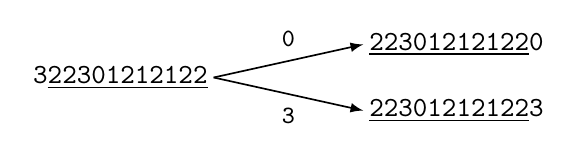
\begin{tikzpicture}[baseline=(source.base),>=latex]
  \node[anchor=east,inner sep=2pt] (source) at (0,0)
    {\texttt{3\underline{22301212122}}};
  \node[anchor=west,inner sep=2pt] (zero) at (1.9,.42)
    {\texttt{\underline{22301212122}0}};
  \node[anchor=west,inner sep=2pt] (three) at (1.9,-.42)
    {\texttt{\underline{22301212122}3}};
  \draw[->,semithick] (source.east) --
    node[midway,above=4pt,inner sep=1pt,font=\small] {\texttt{0}} (zero.west);
  \draw[->,semithick] (source.east) --
    node[midway,below=4pt,inner sep=1pt,font=\small] {\texttt{3}} (three.west);
 \end{tikzpicture}
\]
The calculation therefore continues with two queues, $\mathtt{20}$
and $\mathtt{23}$. On the board $\sigma_{33}=\mathtt{0}$, so the first queue
is the actual one; the second is an extra possibility allowed by
the graph.

\medskip\noindent
\textbf{Checking the new symbol.}
The graph is used a second time, at the other end of the word.
We say that a word $\sigma_1\dots\sigma_T$, with $T\ge12$,
\emph{follows the history graph} if every window
$\sigma_{t-11}\dots\sigma_t$ with $12\le t\le T$ is a vertex, and
for $12\le t<T$ there is an edge
\[
 \sigma_{t-11}\dots\sigma_t\xrightarrow{\;\sigma_{t+1}\;}
 \sigma_{t-10}\dots\sigma_{t+1}.
\]
Once the calculation has chosen the queen in column $n$, it produces
the new symbol $\sigma_n$ (Section~\ref{app:output}). If
$\sigma_1\dots\sigma_{n-1}$ follows the graph, its last window is
$H_{\mathrm{out}}=\sigma_{n-12}\dots\sigma_{n-1}$, so
$\sigma_1\dots\sigma_n$ follows the graph exactly when
$H_{\mathrm{out}}$ has an outgoing edge labeled $\sigma_n$. The
\emph{output check} confirms that this edge exists; the calculation
then replaces $H_{\mathrm{out}}$ by its destination. It is the second
stage of the step in Section~\ref{app:output}. This is why the
state stores $H_{\mathrm{out}}$: on the board, it is the vertex at
which the walk of the queen word currently ends.

\medskip\noindent
\textbf{The branch that describes the board.}
The two uses fit together. On the board, every requested symbol has
index below $n$ (Lemma~\ref{lem:local-exactness}), so it belongs to
$\sigma_1\dots\sigma_{n-1}$. Section~\ref{sec:identification} proves
by induction that this prefix follows the graph, so each requested
symbol labels an edge leaving the vertex from which it is read. The
branch that answers each request with the actual symbol of the queen
word therefore never stops
for lack of an edge, and Section~\ref{sec:sufficiency} shows that it
produces the actual next queen and records. Its output check extends
the walk of the queen word by one symbol, so the requests made in
the next column are covered in turn.

\medskip\noindent
\textbf{The other branches.}
The graph allows more than the queen word does: it has vertices that
never occur as subwords of~$\sigma$, and edges that $\sigma$ never
uses. The calculation follows every edge and cannot tell which
branch is the actual one. In particular, it never compares the
symbols it reads with those in $H_{\mathrm{out}}$, although on the
board the two can overlap: in the column-$41$ example, $\sigma_{29}$
is both the last symbol of $Q$ and the first symbol of
$H_{\mathrm{out}}$. The other branches are not discarded. Each one
that does not stop must still pass the output check and give a
successor satisfying the bounds of Section~\ref{sec:sufficiency};
Section~\ref{sec:finite} verifies this for every branch. With the
graph we use, no branch ever stops for lack of an edge
(Section~\ref{sec:closure-check}).


\subsection{Recovering the upper attacks and counts}\label{app:upper}

The sets $R,D,A$ decide which lower candidates are attacked by lower
queens. An upper queen in row $m+r$ appears as the bit $b_{m+r}=1$ in
the queue, requested from the history graph if necessary. Two
questions about upper queens remain:
\begin{enumerate}
\item Does an upper queen attack a candidate $(n,m+r)$ along its
antidiagonal?
\item Does row $n$ contain an upper queen? This is the bit $b_n$
needed for the new symbol $\sigma_n=2u_n+b_n$.
\end{enumerate}
Propositions~\ref{prop:upper-antidiagonal-test}
and~\ref{prop:upper-row-count} answer both questions using only the
stored words and $z$. Their derivations refer to the actual board.
Both answers take into account only the upper queens in columns
whose symbols are stored in $H_{\mathrm{in}}$ and $Q$;
Section~\ref{sec:sufficiency} shows that, after the requests made in
Section~\ref{app:output}, no other upper queen can affect either
answer.

\medskip\noindent
\textbf{The columns represented by the stored symbols.}
Write a column as $m+h$, so that $h$ is its offset from $m$. The
symbols of $H_{\mathrm{in}}$ belong to columns $m-12,\dots,m-1$, and
those of $Q$ to columns $m,\dots,m+|Q|-1$. We call
\[
 h\in[-12\dts|Q|-1]
\]
the \emph{retained offsets}: for each of them the symbol of column
$m+h$ is stored, so the calculation can read $u_{m+h}$. Each request
adds the next nonnegative offset.

\medskip\noindent
\textbf{Relative upper-queen positions.}
By Lemma~\ref{lem:upper}, the upper queen in column $c$ has row
$c+U(c)$. The state stores neither the column nor the growing count
$U(c)$, so we measure both from a common reference. Write
$\kappa=U(m-1)$ for the number of upper queens in columns less than $m$.
Like $n$ and $m$, it is used only to interpret the records; the
calculation never computes it. For a retained offset $h$, the
difference $\Gamma(h)=U(m+h)-\kappa$ is a count of stored
column bits:
\begin{equation}\label{eq:C}
 \Gamma(h)=
 \begin{cases}
  \displaystyle\sum_{i=0}^{h}u_{m+i},&h\ge0,\\[4pt]
  \displaystyle-\sum_{i=h+1}^{-1}u_{m+i},&h<0.
 \end{cases}
\end{equation}
For $h\ge0$ it counts the upper columns $m,\dots,m+h$; for $h<0$ it
subtracts the upper columns $m+h+1,\dots,m-1$, so that
$\Gamma(-1)=0$. Substituting $U(m+h)=\kappa+\Gamma(h)$ into
Lemma~\ref{lem:upper}, the upper queen in column $m+h$, when
$u_{m+h}=1$, has
\begin{equation}\label{eq:source-offsets}
 \begin{array}{ll}
 \text{row}&m+\kappa+h+\Gamma(h),\\
 \text{antidiagonal index}&2m+\kappa+2h+\Gamma(h).
 \end{array}
\end{equation}
The terms $h+\Gamma(h)$ and $2h+\Gamma(h)$ can be computed from the
stored symbols; the references $m+\kappa$ and $2m+\kappa$ will cancel
from both tests. For example, before column $41$ we have $m=25$ and
$\kappa=16$. Among columns $25,26,27$, only $27$ is upper, so
$\Gamma(2)=1$, and the queen in column $27$ has row
$25+16+2+1=44$.

\medskip\noindent
\textbf{Locating the current column.}
Both tests compare an upper queen with a position involving the
current column $n$. This is why the state stores $z=n-m-\kappa$
(Definition~\ref{def:local-state}): in the same coordinates,
\begin{equation}\label{eq:relative}
 n=m+\kappa+z.
\end{equation}
In the column-$41$ example, $z=41-25-16=0$.

\begin{proposition}[Upper-antidiagonal attack criterion]\label{prop:upper-antidiagonal-test}
Fix a lower candidate $(n,m+r)$, where $0\le r\le w$.
Let $m+h$ be an upper column represented in $H_{\mathrm{in}}$
or $Q$, so $h\in[-12\dts |Q|-1]$ and $u_{m+h}=1$.
The upper queen in column $m+h$ attacks the candidate along
its antidiagonal if and only if
\begin{equation}\label{eq:upper-sum}
 2h+\Gamma(h)=z+r.
\end{equation}
\end{proposition}

\begin{proof}
By \eqref{eq:source-offsets}, the upper queen's antidiagonal
index is $2m+\kappa+2h+\Gamma(h)$. The candidate's is
\[
 n+m+r=2m+\kappa+z+r.
\]
The two squares lie on the same antidiagonal precisely when
these indices agree. Canceling $2m+\kappa$ gives
\eqref{eq:upper-sum}.
\end{proof}

\medskip\noindent
\textbf{Counting upper rows to determine the new bit.}
Once the queen in column $n$ has been chosen, $u_n$ is known, and it
remains to find $b_n$. Write
\[
 B(T)=\sum_{i=1}^{T}b_i
\]
for the number of upper queens in rows at most $T$. Then
$b_n=B(n)-B(n-1)$, so it suffices to compute $B$ at the two
thresholds $n-1$ and $n$.

The count $\kappa$ includes upper queens according to their
\emph{columns}: exactly those in columns less than $m$. To count them by
their \emph{rows} instead, start from $\kappa$ and make two
adjustments:
\begin{itemize}
\item subtract the upper queens in columns less than $m$ whose rows are
greater than $T$;
\item add the upper queens in columns at least $m$ whose rows are at
most $T$.
\end{itemize}
Thus
\begin{equation}\label{eq:upper-row-adjustment}
 \begin{split}
 B(T)={}&\kappa-\#\{1\le c<m:u_c=1,\ q_c>T\}\\
        &+\#\{c\ge m:u_c=1,\ q_c\le T\}.
 \end{split}
\end{equation}

\begin{figure}[!htbp]
\centering
\begin{tikzpicture}[font=\small]
 \foreach \xx/\threshold/\caseTitle in {0/0/{Subtract from $\kappa$},7.65/2.0125/{Add to $\kappa$}} {
  \begin{scope}[xshift=\xx cm,x=.82cm,y=.84cm]
   \setboardfontsize{9pt}
   \node[font=\small\bfseries] at (-.3,4.0) {\caseTitle};
   % The same queens and column cut, with two different row thresholds.
   \draw[black!65,line width=.65pt] (0,-2.27)--(0,2.65);
   \draw[black!65,line width=.65pt] (-2.95,\threshold)--(2.75,\threshold);
   \node[anchor=north] at (0,-2.43) {$m$};
   \node[anchor=west] at (2.87,\threshold) {$T$};

   % A rescaled stretch of actual upper queens: (1,2), (2,4),
   % (5,8), (6,10), (7,12), (8,14), (11,18).
   \foreach \c/\r in {-2.60/-2.0125,-2.20/-1.4375,-1.00/-.2875,
                       -.60/.2875,-.20/.8625,.20/1.4375,1.40/2.5875} {
    \ifdim\r pt>\threshold pt
     \ifdim\c pt<0pt \def\qcolor{black!55}\else\def\qcolor{black!30}\fi
    \else \def\qcolor{queensUpper}\fi
    \node[text=\qcolor,inner sep=0pt] at (\c,\r) {\BlackQueenOnWhite};
   }

   \draw[decorate,decoration={brace,amplitude=4pt},black!65]
    (-2.95,2.52)--(-.12,2.52);
   \node[anchor=south] at (-1.535,2.81) {$\kappa=U(m-1)$};
   \draw[decorate,decoration={brace,amplitude=4pt},black!65]
    (-3.20,-2.16)--(-3.20,{\threshold-.08});
   \node[anchor=east] at (-3.48,{(\threshold-2.24)/2}) {$B(T)$};
  \end{scope}
 }
\end{tikzpicture}
\caption{The adjustments in \eqref{eq:upper-row-adjustment}. Left:
upper queens left of $m$ and above $T$ are subtracted from $\kappa$.
Right: those right of $m$ and at or below $T$ are added. Upper-queen
rows increase with their columns (Lemma~\ref{lem:upper}), so at most
one adjustment is nonzero. Teal queens are counted by $B(T)$.}
\label{fig:row-count-adjustment}
\end{figure}


For instance, on the column-$41$ board, counting upper rows through
$T=39$ means subtracting the queen at $(24,40)$ from the sixteen
counted by $\kappa$, with nothing to add, so $B(39)=15$.

For an upper queen in a retained column, the comparison with $T$ can
be made from the stored symbols. Write the threshold as
$T=m+\kappa+x$. By \eqref{eq:source-offsets}, the queen in column
$m+h$ has row $m+\kappa+h+\Gamma(h)$, so it lies at or below row $T$
exactly when $h+\Gamma(h)\le x$. Let $\J(x)$ be the net adjustment
computed from the retained columns, with additions from $Q$ and
subtractions from $H_{\mathrm{in}}$:
\begin{equation}\label{eq:J}
 \begin{split}
 \J(x)={}&\#\{0\le h<|Q|:u_{m+h}=1,\ h+\Gamma(h)\le x\}\\
 &-\#\{-12\le h<0:u_{m+h}=1,\ h+\Gamma(h)>x\}.
 \end{split}
\end{equation}

\begin{proposition}[Upper-row counting formula]\label{prop:upper-row-count}
Fix a nonnegative integer threshold $T$ and write
$T=m+\kappa+x$. Suppose that every upper queen in a column
less than $m-12$ lies at or below row $T$, and every upper
queen in a column at least $m+|Q|$ lies above row $T$. Then
\[
 B(T)=\kappa+\J(x).
\]
If these assumptions hold for both $T=n-1$ and $T=n$, then
\begin{equation}\label{eq:J-count}
 B(n-1)=\kappa+\J(z-1),\qquad B(n)=\kappa+\J(z),
\end{equation}
and hence
\[
 b_n=\J(z)-\J(z-1).
\]
\end{proposition}

\begin{proof}
In \eqref{eq:upper-row-adjustment}, the first assumption means
that no upper queen before column $m-12$ needs to be subtracted.
Every required subtraction is therefore represented in
$H_{\mathrm{in}}$. The second assumption means that no upper
queen in column $m+|Q|$ or later needs to be added, so every
required addition is represented in $Q$. The two adjustments
are exactly the two terms defining $\J(x)$ in \eqref{eq:J}.
This proves $B(T)=\kappa+\J(x)$.

Since $n=m+\kappa+z$, the thresholds $T=n-1,n$ correspond
to $x=z-1,z$, respectively. Substituting these values gives
\eqref{eq:J-count}. Taking the difference cancels $\kappa$
and gives the stated formula for $b_n$.
\end{proof}

The calculation therefore finds $b_n$ from the two adjustments
$\J(z-1)$ and $\J(z)$, without knowing $\kappa$. Neither $\Gamma$ nor
$\J$ is stored; both are computed from the stored words when needed.

\subsection{The calculation}\label{app:output}

We now give the whole calculation on a state before column $n$. It
has four stages: choose the queen, produce and check the new symbol
$\sigma_n$, update the row and diagonal references, and update the
input words. Whenever a stage needs a symbol beyond the end of $Q$,
the calculation makes a request, answered from the history graph as
in Section~\ref{app:graph}. This may split the calculation into
branches, and the remaining stages are carried out separately in
each branch. Symbols appended to $Q$ stay there for the rest of the
branch, even if the candidate that needed them is rejected.
Throughout, $u_{m+h}$ and $b_{m+h}$ denote the two bits of the stored
symbol at offset $h$; the calculation never uses the values of $n$,
$m$, or $d$.

Before choosing the queen, extend $Q$ by requests, if necessary, to
length at least $z$. This supplies the symbols needed later for
$\J(z-1)$ and $\J(z)$.

\medskip\noindent
\textbf{Choose the queen.}
The lower candidates are $(n,m+r)$ for $r=0,\dots,w$; there are none
when $w<0$. Test them in increasing order of $r$, so that the first
one accepted is the lowest. First test attacks from lower queens:
reject the candidate if $r\in R$, $w-r\in D$, or $r\in A$. 
A~candidate that passes these three tests is then tested for upper
attacks along its row and antidiagonal. The row test reads
$b_{m+r}$, the row bit at offset $r$. By
Proposition~\ref{prop:upper-antidiagonal-test}, the upper queen in
column $m+h$ attacks along the antidiagonal only if
$2h+\Gamma(h)=z+r$. For $h\ge0$ we have $\Gamma(h)\ge0$, so such an
offset satisfies $h\le\lfloor(z+r)/2\rfloor$; the negative retained
offsets are already stored in $H_{\mathrm{in}}$. Both tests are
therefore covered by extending $Q$, if necessary, to length at least
\[
 1+\max\{r,\lfloor(z+r)/2\rfloor\}.
\]
Reject the candidate if $b_{m+r}=1$, or if some retained offset $h$
with $u_{m+h}=1$ satisfies \eqref{eq:upper-sum}. Choose the first
candidate that passes all five tests. If there are no candidates, or
all are rejected, choose an upper queen. Knuth's \texttt{infty-queens} program \cite{KnuthQueens} also tries
the lower candidates first and places an upper queen only when all of
them are attacked; here the tests use only the local records.

\medskip\noindent
\textbf{Produce and check the new symbol.}
The choice gives $u_n=1$ if the queen is upper and $u_n=0$ if it is
lower. Following Proposition~\ref{prop:upper-row-count}, the
calculation computes
\begin{equation}\label{eq:output}
 b_{\mathrm{out}}=\J(z)-\J(z-1),\qquad
 s=2u_n+b_{\mathrm{out}}.
\end{equation}
It then performs the output check: it confirms that $s$ labels an
edge leaving $H_{\mathrm{out}}$, and
replaces $H_{\mathrm{out}}$ by $\last(H_{\mathrm{out}}s)$. In the
exhaustive check of Section~\ref{sec:closure-check}, a missing output edge in any
branch makes the whole verification fail.

\medskip\noindent
\textbf{Update the row and diagonal references.}
Placing the queen may use up the least unused row $m$ or the least
unused magnitude $d$, so the next state measures its records from
new reference values. First record the queen if it is lower, by
inserting $r$, $w-r$, and $r$ into $R$, $D$, and $A$; an upper queen
adds nothing, since these sets record only lower queens. Write
$\widetilde R,\widetilde D,\widetilde A$ for the resulting sets.
Write $\mu$ and $\nu$ for the advances of the row and diagonal
references, so that the new least unused row is $m+\mu$ and the new
least unused magnitude is $d+\nu$. Measured from the current
references $m$ and $d$, row $m+h$ is used when a recorded lower queen
($h\in\widetilde R$) or an upper queen ($b_{m+h}=1$) occupies it, and
magnitude $d+h$ is used when $h\in\widetilde D$; upper queens lie on
no lower diagonal. Hence
\[
 \mu=\min\{h\ge0:h\notin\widetilde R,\ b_{m+h}=0\},\qquad
 \nu=\min(\N\setminus\widetilde D).
\]
The search for $\mu$ reads $b_{m+h}$ for $h=0,\dots,\mu$, making
requests when necessary; the zero bit at offset $\mu$ confirms that
this row is unused. When the new queen is upper,
Section~\ref{sec:sufficiency} proves that the search stops below its
row.

The new references are $n+1$, $m+\mu$, and $d+\nu$. Measuring each
recorded position from its new reference, and discarding offsets
that become negative, gives
\begin{equation}\label{eq:update}
 \begin{aligned}
 w'&=w+1-\mu-\nu,\\
 z'&=z+1-\mu-\textstyle\sum_{h=0}^{\mu-1}u_{m+h},\\
 R'&=\{a-\mu:a\in\widetilde R,\ a\ge\mu\},\\
 D'&=\{a-\nu:a\in\widetilde D,\ a\ge\nu\},\\
 A'&=\{a-(1+\mu):a\in\widetilde A,\ a\ge1+\mu\}.
 \end{aligned}
\end{equation}
The formula for $w'$ follows from $w=n-m-d$. For $z=n-m-U(m-1)$, the
column advances by one and the row reference by $\mu$, while
$U(m+\mu-1)$ exceeds $U(m-1)$ by the number of upper columns among
$m,\dots,m+\mu-1$; the row search has read all of their symbols. The
antidiagonal reference $n+m$ advances by $1+\mu$. Discarding negative
offsets loses nothing: the references $m$, $d$, and $n+m$ never
decrease, so a row, diagonal, or antidiagonal whose index has fallen
below its reference cannot contain a later candidate.

\medskip\noindent
\textbf{Update the input words.}
The input history must now end at index $m+\mu-1$, and the queue
must begin at index $m+\mu$. Remove the first $\mu$ symbols of the
extended $Q$ and append them to $H_{\mathrm{in}}$, keeping its last
twelve symbols. The symbol at offset $\mu$ stays as the first symbol
of $Q'$, so $Q'$ is nonempty. These two words, together with
$w',z',R',D',A'$ and the new output history, form the successor
state.

\medskip
Algorithm~\ref{alg:local-successors} collects the four stages. It
follows a single branch: $Q$ denotes the queue of that branch, which
grows as requests are made, and \Call{Extend}{$k$} makes requests
until $|Q|\ge k$. Each request may split the calculation, as
described in Section~\ref{app:graph}, and a request at a vertex
without outgoing edges stops the branch. In the column-$53$ example
of that section, \Call{Extend}{$2$} makes one request, for
$\sigma_{33}$, which splits the calculation into branches with queues
$\mathtt{20}$ and $\mathtt{23}$. The successors of a state are the
states returned by all of its branches that do not stop. In the
listing, $\J$ and $\Gamma$ are computed from $H_{\mathrm{in}}$ and the
current $Q$.

\begin{algorithm}[H]
\caption{One branch of the calculation}
\label{alg:local-successors}
\renewcommand{\algorithmicrequire}{\textbf{Input:}}
\renewcommand{\algorithmicensure}{\textbf{Output:}}
\begin{algorithmic}[1]
\Require The history graph and a state $(w,z,R,D,A,H_{\mathrm{in}},Q,H_{\mathrm{out}})$.
\Ensure A successor state; failure if the output check fails; nothing if the branch stops.
\State \Call{Extend}{$z$}\Comment{prepare for $\J(z-1),\J(z)$}
\State $c\gets\texttt{UPPER}$; $r\gets0$\Comment{choose the queen}
\While{$c=\texttt{UPPER}$ and $r\le w$}
  \If{$r\notin R$ and $w-r\notin D$ and $r\notin A$}\Comment{no lower-queen attack}
    \State \Call{Extend}{$1+\max\{r,\lfloor(z+r)/2\rfloor\}$}\Comment{reach the symbols the tests need}
    \If{$b_{m+r}=0$ and no retained offset $h$ with $u_{m+h}=1$ has $2h+\Gamma(h)=z+r$}
      \State $c\gets r$\Comment{no upper-queen attack}
    \EndIf
  \EndIf
  \State $r\gets r+1$
\EndWhile
\State Set $u_n\gets1$ if $c=\texttt{UPPER}$ and $u_n\gets0$ otherwise.\Comment{produce the new symbol}
\State Compute $b_{\mathrm{out}}$ and $s$ by \eqref{eq:output}.
\If{$H_{\mathrm{out}}$ has no outgoing edge labeled $s$}\Comment{output check}
  \State \Return failure
\EndIf
\State $H'_{\mathrm{out}}\gets\last(H_{\mathrm{out}}s)$.
\State Form $\widetilde R,\widetilde D,\widetilde A$, inserting $c,w-c,c$ if $c\ne\texttt{UPPER}$.\Comment{update the references}
\State $\nu\gets\min(\N\setminus\widetilde D)$; $\mu\gets0$.
\While{$\mu\in\widetilde R$ or $b_{m+\mu}=1$}\Comment{row $m+\mu$ is used}
  \State $\mu\gets\mu+1$; \Call{Extend}{$\mu+1$}.
\EndWhile
\State Compute $w',z',R',D',A'$ by \eqref{eq:update}.
\State Split $Q=PQ'$ with $|P|=\mu$, and set $H'_{\mathrm{in}}\gets\last(H_{\mathrm{in}}P)$.\Comment{update the input words}
\State \Return $(w',z',R',D',A',H'_{\mathrm{in}},Q',H'_{\mathrm{out}})$
\end{algorithmic}
\end{algorithm}

Starting from the state before column $30$
(Section~\ref{app:seed}) and applying the calculation to each
successor in turn produces a directed graph of states, which
Section~\ref{sec:finite} examines exhaustively.

\begin{definition}[State graph]\label{def:state-graph}
The \emph{state graph} has as vertices the
states reached from the state before column $30$ by repeating the
calculation. It has a directed edge $S\to S'$ when some branch of
the calculation on $S$ produces $S'$.
\end{definition}

Different branches may produce the same successor; they then give a
single edge. Section~\ref{sec:finite} verifies that every output
check passes, that every successor satisfies
Condition~\ref{cond:state}, and that only finitely many states are
reached. Note that the definition assumes none of these properties.

\subsection{Worked examples of the state transition}\label{sec:worked-transition}

We first carry out the complete calculation for column $41$,
starting from the state of Figure~\ref{fig:state-portrait}:
\[
 \begin{gathered}
 w=2,\qquad z=0,\qquad R=A=\varnothing,\qquad D=\{1,2\},\\
 H_{\mathrm{in}}=\mathtt{212223003223},\qquad Q=\mathtt{01212},\\
 H_{\mathrm{out}}=\mathtt{212203230303}.
 \end{gathered}
\]
The three words hold indices $13$--$24$, $25$--$29$, and $29$--$40$.
We use the board values $n=41$, $m=25$, $d=14$, and $\kappa=16$ only
to explain the numbers; they are not stored. The queue already
contains every symbol this step needs, so the calculation makes no
request and does not branch. Afterwards we look briefly at three
further steps: one in which the input words move, one in which an
upper attack rules out the only lower candidate, and one in which
the calculation branches.

\medskip\noindent
\textbf{Choose the queen.}
Since $w=2$, the lower candidates have offsets $r=0,1,2$, in rows
$25,26,27$. Since $R$ and $A$ are empty, no lower queen attacks a
candidate along its row or antidiagonal. The lower-diagonal test
gives
\begin{center}
\begin{tabular}{clcl}
\toprule
$r$&Candidate&$w-r$&Lower-diagonal test\\
\midrule
$0$&$(41,25)$&$2$&Reject: $2\in D$\\
$1$&$(41,26)$&$1$&Reject: $1\in D$\\
$2$&$(41,27)$&$0$&Pass: $0\notin D$\\
\bottomrule
\end{tabular}
\end{center}
Only $(41,27)$ reaches the upper tests. Its row bit $b_{27}$ comes
from $\sigma_{27}=\mathtt{2}$ and is zero. An antidiagonal attack needs
an upper column with
\[
 2h+\Gamma(h)=z+r=2.
\]
The upper columns in $H_{\mathrm{in}}$ have $h<0$ and $\Gamma(h)\le0$,
so for them $2h+\Gamma(h)\le-2$. In $Q=\mathtt{01212}$, the upper
columns are at offsets $h=2,4$, with $\Gamma(h)=1,2$, giving
$2h+\Gamma(h)=5$ and $10$. The candidate passes all five tests, and the queen is placed
at $(41,27)$. It is the $j=d+|D|=16$th lower queen, with magnitude
$14$, so \eqref{eq:local-rank} gives the discrepancy bounded by
Lemma~\ref{lem:estimates}:
\[
 d_j-j=w-r-|D|=2-2-2=-2.
\]

\medskip\noindent
\textbf{Produce and check the new symbol.}
The queen is lower, so $u_{41}=0$. Since $z=0$, the new row bit $b_{41}$
comes from $\J(-1)$ and $\J(0)$. The upper columns in $H_{\mathrm{in}}$
have relative rows $h+\Gamma(h)\le-1$, so neither $\J(-1)$ nor
$\J(0)$ subtracts them. Those in $Q$ have relative rows $2+1=3$ and
$4+2=6$, so neither adds them either. Hence
\[
 \J(-1)=\J(0)=0,\qquad
 b_{\mathrm{out}}=0-0=0,\qquad s=2\cdot0+0=0.
\]
On the board the two thresholds are rows $40$ and $41$. The upper
rows nearest them are $40$ and $44$, so $B(40)=B(41)$, which is why
$b_{41}=0$. The output check
succeeds, since the history graph has the edge
\[
 \mathtt{212203230303}\xrightarrow{\;\texttt{0}\;}
 \mathtt{122032303030},
\]
and $H_{\mathrm{out}}$ becomes its destination.

\medskip\noindent
\textbf{Update the row and diagonal references.}
The new queen has row $27$, lower-diagonal magnitude $14$, and
antidiagonal index $68$. Their offsets from the references
$25,14,66$ are $2,0,2$, so
\[
 \widetilde R=\{2\},\qquad
 \widetilde D=\{0,1,2\},\qquad
 \widetilde A=\{2\}.
\]
Row $25$ is still unused: the candidate $(41,25)$ was rejected
because of a diagonal attack, not because its row was occupied.
Hence $\mu=0$. Magnitude $14$ fills the gap below the used
magnitudes $15$ and $16$, so the least unused magnitude becomes $17$
and $\nu=3$. By \eqref{eq:update},
\[
 R'=\{2\},\qquad D'=\varnothing,\qquad A'=\{1\},\qquad
 w'=2+1-0-3=0,\qquad z'=0+1-0-0=1.
\]
All three offsets in $\widetilde D$ are discarded, because the
magnitudes $14,15,16$ now lie below the reference $17$. On the board,
$w'=42-25-17=0$ and $z'=42-25-16=1$, so column $42$ has the single
lower candidate $(42,25)$.

\medskip\noindent
\textbf{Update the input words.}
Since $\mu=0$, no symbols move, and $H_{\mathrm{in}}$ and $Q$ are
unchanged. Table~\ref{tab:local-transition} summarizes the step,
which is one edge of the state graph.
\begin{table}[!htbp]
\centering
\begin{tabular}{lll}
\toprule
Field&Before column $41$&Before column $42$\\
\midrule
$w$&$2$&$0$\\
$z$&$0$&$1$\\
$R$&$\varnothing$&$\{2\}$\\
$D$&$\{1,2\}$&$\varnothing$\\
$A$&$\varnothing$&$\{1\}$\\
$H_{\mathrm{in}}$&\texttt{212223003223}&\texttt{212223003223}\\
$Q$&\texttt{01212}&\texttt{01212}\\
$H_{\mathrm{out}}$&\texttt{212203230303}&\texttt{122032303030}\\
\bottomrule
\end{tabular}
\caption{One edge of the state graph. The input words do not move
because the least unused row is still $25$; the output history
shifts and appends $\mathtt{0}$.}\label{tab:local-transition}
\end{table}

\medskip\noindent
\textbf{When the input words move: column $42$.}
The sole lower candidate $(42,25)$ passes all five tests. After it is
placed, the search for the least unused row passes rows $25$
through $28$, occupied respectively by the new lower queen, an upper
queen, the queen placed in column $41$, and an upper queen. Row $29$
is unused, so $\mu=4$. The first four symbols $\mathtt{0121}$ of
$Q=\mathtt{01212}$, for indices $25$ through $28$, move into
$H_{\mathrm{in}}$:
\[
 \begin{aligned}
 H'_{\mathrm{in}}&=\last(H_{\mathrm{in}}\,\mathtt{0121})
                  =\mathtt{230032230121},\\
 Q'&=\mathtt{2}.
 \end{aligned}
\]
The new input history covers indices $17$ through $28$, and
$Q'=\sigma_{29}$, whose zero row bit confirms that row $29$ is
unused. Among the moved symbols only $\sigma_{27}=\mathtt{2}$ is upper, so
$z'=1+1-4-1=-3$, in agreement with $43-29-U(28)=43-29-17$. No
request was needed: the step moved symbols already in $Q$.

\medskip\noindent
\textbf{When a lower candidate is attacked: column $47$.}
Before column $47$, we have $m=29$, $w=0$, $z=1$, and
$R=D=A=\varnothing$. The sole lower candidate $(47,29)$ passes the
three lower-queen tests, and $Q=\mathtt{2}$ gives $b_{29}=0$, so no
upper queen occupies its row. However, the upper queen $(29,47)$
shares its antidiagonal $76$. This queen has offset $h=0$ and
$\Gamma(0)=1$, so \eqref{eq:upper-sum} holds: $2h+\Gamma(h)=1=z+r$
with $r=0$. The candidate is rejected, and the $30$th upper queen is
placed at $(47,77)$. Thus a nonempty candidate interval can still
end with an upper queen.

\medskip\noindent
\textbf{When the calculation branches: column $53$.}
As in Section~\ref{app:graph}, before column $53$ we have $m=32$,
$Q=\mathtt{2}$, and $z=2$. The calculation first extends $Q$ to
length two, and the vertex $\mathtt{322301212122}$ has two outgoing
edges, giving two branches with queues $\mathtt{20}$ and
$\mathtt{23}$. The appended symbols are the two values allowed for
the earlier symbol $\sigma_{33}$, not choices of a queen in
column $53$.

Both branches choose the lower square $(53,32)$ and produce
$\sigma_{53}=\mathtt{0}$, but their record updates differ. With
$Q=\mathtt{20}$, the row bit at index $33$ is zero, so the next
unused row is $33$ and $\mu=1$. With $Q=\mathtt{23}$, that bit is
one, and the row search makes another request. The vertex reached
has a single outgoing edge, labeled $\mathtt{0}$, so $Q=\mathtt{230}$ and the
search stops at row $34$, giving $\mu=2$. The two branches therefore
produce different successors, although they chose the same queen and
produced the same symbol. On the board $\sigma_{33}=\mathtt{0}$, so the first
branch gives the actual next state; the verification checks the
second as well.
